\subsection{Task 2: Pagerank}
In this experiment, we run pagerank on various size of graph data.

\subsubsection{Plot}

\begin{figure}[h]
\begin{center}
\begin{tabular}{cc}
     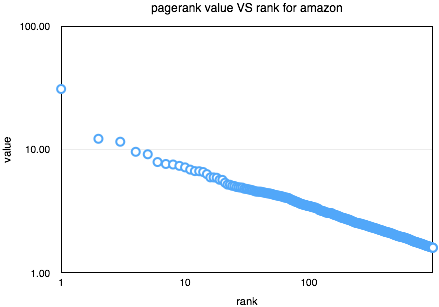
\includegraphics[width=0.4\textwidth]{FIG/t2_amazon.png} &
     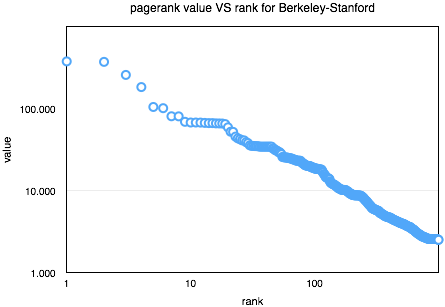
\includegraphics[width=0.4\textwidth]{FIG/t2_berke.png} \\
    (a) & (b) 
\end{tabular}
\caption{(a)Amazon (b)Berkeley-Stanford web graph}
\label{t2:1}
\end{center}
\end{figure}

\begin{figure}[h]
\begin{center}
\begin{tabular}{cc}
     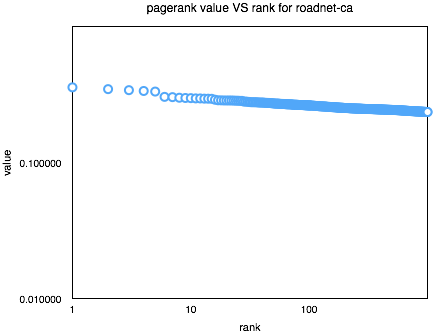
\includegraphics[width=0.4\textwidth]{FIG/t2_ca.png} &
     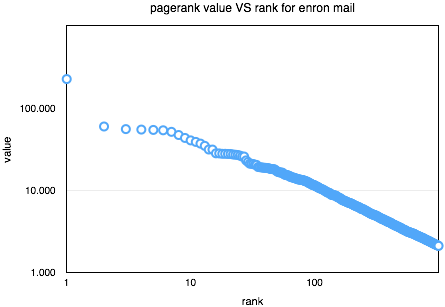
\includegraphics[width=0.4\textwidth]{FIG/t2_enron.png} \\
    (a) & (b) 
\end{tabular}
\caption{(a)Roadnet-CA (b)Enron Mail}
\label{t2:2}
\end{center}
\end{figure}

\begin{figure}[h]
\begin{center}
\begin{tabular}{cc}
     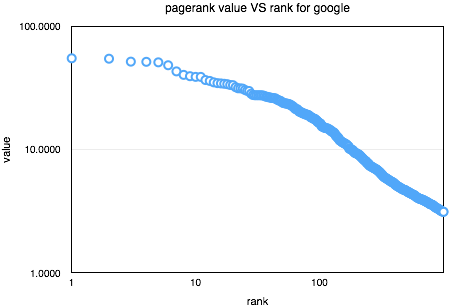
\includegraphics[width=0.4\textwidth]{FIG/t2_google.png} &
     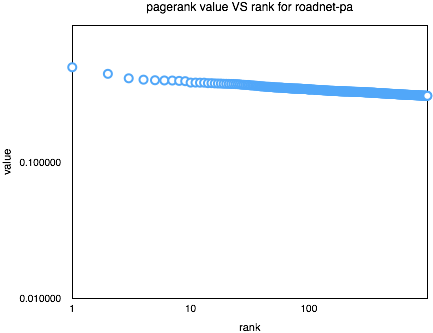
\includegraphics[width=0.4\textwidth]{FIG/t2_pa.png} \\
    (a) & (b) 
\end{tabular}
\caption{(a)Google web graph (b)Roadnet-PA}
\label{t2:3}
\end{center}
\end{figure}

\begin{figure}[h]
\begin{center}
\begin{tabular}{cc}
     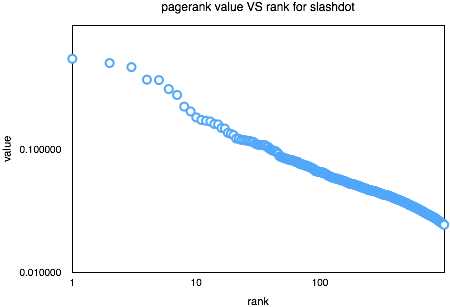
\includegraphics[width=0.4\textwidth]{FIG/t2_slashdot.png} &
     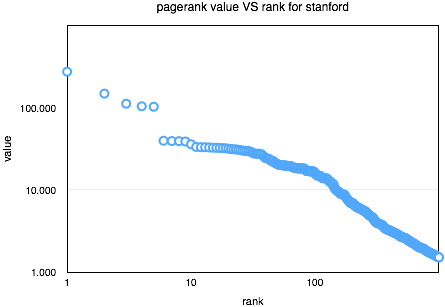
\includegraphics[width=0.4\textwidth]{FIG/t2_stanford.png} \\
    (a) & (b) 
\end{tabular}
\caption{(a)Slashdot (b)Stanford}
\label{t2:4}
\end{center}
\end{figure}

\begin{figure}[h]
\begin{center}
\begin{tabular}{cc}
     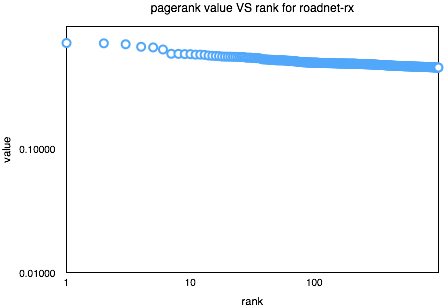
\includegraphics[width=0.4\textwidth]{FIG/t2_tx.png} &
     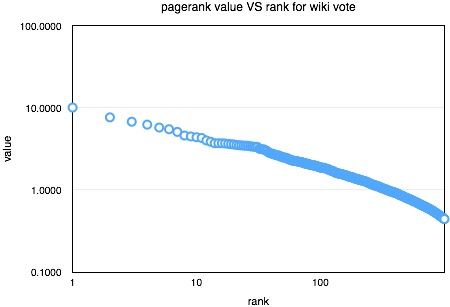
\includegraphics[width=0.4\textwidth]{FIG/t2_wikivote.png} \\
    (a) & (b) 
\end{tabular}
\caption{(a)Roadnet-TX (b)Wiki vote}
\label{t2:5}
\end{center}
\end{figure}


\subsubsection{Observation}






